\def\mya{\theta-\theta(x)}
\def\linex{e^{c(\mya)} - c(\mya) -1}

Consider the LINEX loss function defined by 
\[
  L(\mya) = \linex.
\]
(a) Show that $L(\mya \ge 0 $ and plot this as a function of $(\mya)$ when $c= .1, .5, 1, 2$.\\
(b) Find $\hat\theta(x)$ the estimator that minimizes the Bayesian expected posterior loss.\\
(c) Find $\hat\theta(x)$ when $x_1,...x_n~|~\theta \sim N(\theta,1), \theta \sim N(\mu,\tau^2)$.

\subsection*{Solution:}
\subsubsection*{(a)}
Let $a = \mya$, then $L(\mya) = L(a) = e^a - a - 1$. 
\begin{align*}
  \ds\frac{d}{d a} L(a) &:= 0 \\
  e^a - 1 &= 0 \\
  a &= \ln(1) \\
  a &= 0 \\
\end{align*}

\noindent
So, $L(a)$ reaches a local extrema at $a=0 \Rightarrow L(a) = e^0 - 0 - 1 = 0$. 
That is, there is a local extrema at $(0,0)$.
And since $L''(a) = e^a > 0$, $(0,0)$ is a local minimum.\\

\noindent
Therefore, $L(\mya) \geq 0$.

\beginmyfig
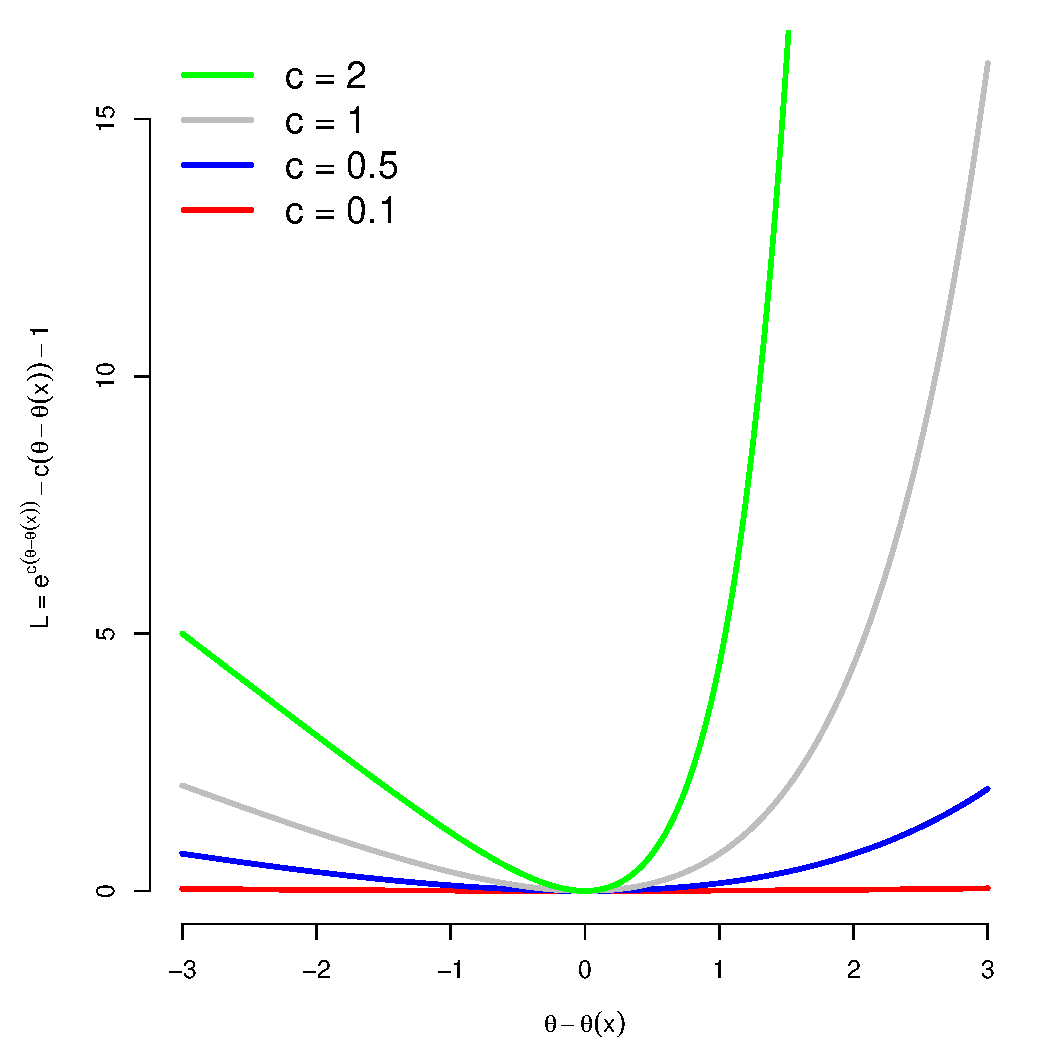
\includegraphics[scale=.7]{../img/fig1.pdf}
\caption{Plot for 7(a). Linex loss as a function of $\theta - \theta(x)$, evaluated at various $c$.}
\endmyfig

\subsubsection*{(b)}
\def\mgf{E_{\theta|x}[e^{c\theta}|x]}
Let $f(\theta|\bm x)$ be the posterior density for $\theta$. Then, the expected
posterior loss is
\begin{align*}
  E[L(\mya)] &= \ds \int_\Theta~\left\{ \linex \right\}f(\theta|x)~d\theta \\
             &= \ds e^{-c\theta(x)}\int_\Theta~e^{c\theta}f(\theta|x)~d\theta - 
                    c\int_\Theta~\theta f(\theta|x)~d\theta +
                    c\theta(x)\int_\Theta~f(\theta|x)~d\theta - 
                    \int_\Theta~f(\theta|x)~d\theta \\\\
             &= e^{-c\theta(x)} \mgf -
                    cE_{\theta|x}[\theta|x] + c\theta(x) - 1\\
                    \\
\end{align*}

To minimize the expected posterior loss,
\begin{align*}
  \ds\frac{d}{d\theta(x)} E[L(\mya)] &:= 0 \\
  -c e^{-c\hat\theta} \mgf + c &= 0 \\
  e^{c\hat\theta} &= \mgf \\
  \\
  \Rightarrow \hat\theta &= \ds\frac{\ln(\mgf)}{c}
\end{align*}

\noindent
This is simply the log of the posterior moment generating function divided by $c$.

\subsubsection*{(c)}
$\hat\theta(x)$ is simply the log of posterior mgf divided by $c$. So, all we 
need to do is compute the posterior of $\theta$.
\def\denom{n\tau^2+1}
\def\postMean{\frac{n\bar{x}\tau^2+\mu}{\denom}}
\def\postVar{\frac{\tau^2}{\denom}}
\begin{align*}
  f_{\theta|\bm x}(\theta|\bm x) &\propto \exp\left\{-\frac{\sum_{i=1}^n(x_i-\theta)^2}{2}\right\}
  \exp\left\{-\frac{(\theta-\mu)^2}{2\tau^2}\right\} \\ 
  &\propto \exp \left\{ \frac{-n\theta^2\tau^2 + 2n\bar{x}\theta\tau^2 -\theta^2 +2\theta\mu}{2\tau^2} \right\} \\
  &\propto \exp \left\{ \frac{-\theta^2(n\tau^2+1)+2\theta(n\bar{x}\tau^2+\mu)}{2\tau^2} \right\}\\
  &\propto \exp\left\{ \frac{\ds-\theta^2+2\theta(\frac{n\bar{x}\tau^2+\mu}{\denom})}{2\frac{\tau^2}{\denom}} \right\}\\
  \\
\Rightarrow \theta|\bm x &\sim N(\tilde{m},\tilde{v}),
\end{align*}
where $\tilde m = \ds\postMean$ and $\tilde v = \ds\postVar$. Finally, using the
MGF of the Normal distribution,

\begin{align*}
  \hat\theta(x) &= \ds\frac{\ln(\exp\left\{ \tilde mc + \tilde vc^2/2 \right\})}{c} \\
                &= \ds\frac{\tilde mc + \tilde vc^2/2}{c} \\
                &= \tilde m + \frac{\tilde vc}{2} \\
                \\
  \Rightarrow \hat\theta(x) &= \frac{(n\bar{x}+c/2)\tau^2+\mu}{\denom} \\
\end{align*}

